\documentclass[parskip=full]{scrartcl}

\usepackage[utf8]{inputenc}			% Umlaute, Sonderzeichen
\usepackage[ngerman]{babel}			% deutsche Sprache
\usepackage{enumitem}				% Listen
\usepackage{graphicx}				% Grafiken
\usepackage{hyperref}				% Hyperlinks
\usepackage[nonumberlist]{glossaries}		% Glossar
\usepackage{amsmath}
\usepackage{pdfpages}				% PDF einbinden


% Hurenkinder und Schusterjungen verhindern
\clubpenalty10000
\widowpenalty10000
\displaywidowpenalty=10000

\DeclareRobustCommand{\glossfirstformat}[1]{\textit{#1}}	% der erste Verweis im Dokument auf ...
\renewcommand*{\glsdisplayfirst}[4]{\glossfirstformat{#1#4}}	% ... einen Glossarbegriff wird kursiv markiert

% Kriterien sollen nicht kursiv erscheinen
\makeatletter
\renewcommand{\@begintheorem}[2]{\trivlist
	\item[\hskip \labelsep{\bfseries #1\ #2}]}
\makeatother


\makenoidxglossaries

\newglossaryentry{EclEmma}{
    name = {EclEmma},
    description = {EclEmma ist ein Plug-In für Eclipse für Code-Überdeckungsanalysen. Es basiert auf JaCoCo. Die hier verwendete Version ist 3.1.2}
}


\subject{FreeJDAQ}
\title{Beschreibung der Grafischen Benutzeroberfläche}
\subtitle{Version 1.0.0}
\author{Leon Huck}
\date{\today}


\begin{document}

%\maketitle

\begin{figure}[htbp]
    \begin{center}
        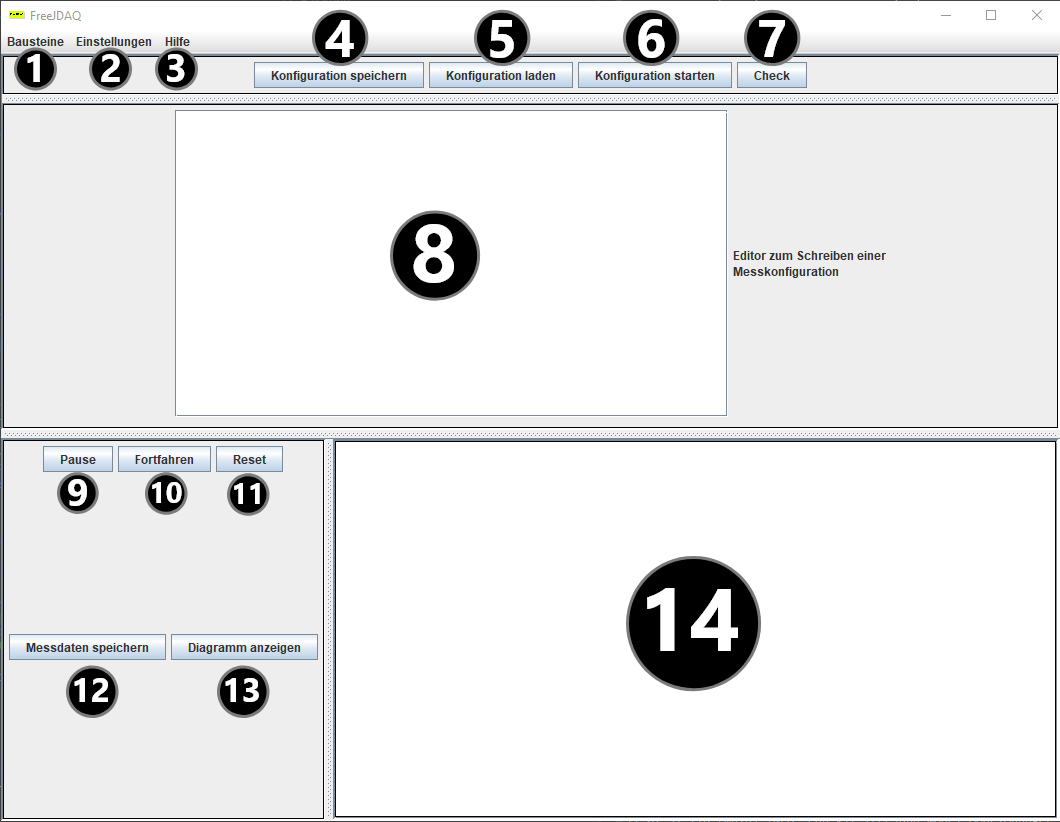
\includegraphics[width = 10cm]{Grafiken/Uebersicht_GUI_Mit_Nummern.png}
        \caption{Die Übersicht über die grafische Benutzeroberfläche von FreeJDAQ. Die Nummern verweißen auf die genauen Beschreibungen, die weiter unten zu finden sind.}
        \label{Uebersicht_GUI_Mit_Nummern}
    \end{center}
\end{figure}

\begin{enumerate}
    \item Bausteine
    Hier muss etwas stehen um den Effekt sehen zu k{\"o}nnen
    \item Einstellungen und Text dahinter
\end{enumerate}

\begin{flushleft}
    
\includegraphics[width = 2cm]{Grafiken/1-Bausteine.png}
\end{flushleft}

\begin{flushleft}
    
\includegraphics[width = 2cm]{Grafiken/2-Einstellungen.png}
\end{flushleft}

\begin{flushleft}
    
\includegraphics[width = 2cm]{Grafiken/3-Hilfe.png}
\end{flushleft}

\begin{flushleft}
    
\includegraphics[width = 2cm]{Grafiken/4-Konfiguration_speichern.png}
\end{flushleft}

\begin{flushleft}
    
\includegraphics[width = 2cm]{Grafiken/5-Konfiguration_laden.png}
\end{flushleft}

\begin{flushleft}
    
\includegraphics[width = 2cm]{Grafiken/6-Konfiguration_starten.png}
\end{flushleft}

\begin{flushleft}
    
\includegraphics[width = 2cm]{Grafiken/7-Check.png}
\end{flushleft}

\begin{flushleft}
    
\includegraphics[width = 2cm]{Grafiken/8-Editor.png}
\end{flushleft}

\begin{flushleft}
    
\includegraphics[width = 2cm]{Grafiken/9-Pause.png}
\end{flushleft}

\begin{flushleft}
    
\includegraphics[width = 2cm]{Grafiken/10-Fortfahren.png}
\end{flushleft}

\begin{flushleft}
    
\includegraphics[width = 2cm]{Grafiken/11-Reset.png}
\end{flushleft}

\begin{flushleft}
    
\includegraphics[width = 2cm]{Grafiken/12-Messdaten_speichern.png}
\end{flushleft}

\begin{flushleft}
    
\includegraphics[width = 2cm]{Grafiken/13-Diagramm_anzeigen.png}
\end{flushleft}

\begin{flushleft}
    
\includegraphics[width = 2cm]{Grafiken/14-Datenanzeige.png}
\end{flushleft}

\end{document}\grid
